% #region PREAMBEL OG PAKKER
\documentclass[a4paper, 12pt]{article}  % DOKUMENTKLASSE
\title{Eksamen ØKO1001\\Del 1: Ledelse} % TITTEL
\author{Kandidatnr. 10026}              % FORFATTER
\date{\today}                           % DATO & FAG

\usepackage[english, norsk]{babel}      % NORSK SPRÅK
\usepackage[                            % BIBLIOGRAFI
    backend=biber,
    style=apa,
    ]{biblatex}
\usepackage{csquotes}                   % PAKKE TIL BABEL
\addbibresource{ref.bib}                % PATH TIL BIBLIOGRAFI
\usepackage[hidelinks]{hyperref}        % LENKER I TOC OG GENERELT
\usepackage[margin=1in]{geometry}       % VANLIG STØRRELSE MARGIN
\setlength{\parindent}{0em}             % SKILLER AVSNITT
\setlength{\parskip}{1em}               % SKILLER AVSNITT
\usepackage{setspace}
\setstretch{1.4}                        % 1.5 LINJEAVSTAND
\usepackage{graphicx}                   % BILDER \includegraphics[OPTIONS]{PATH}
\usepackage{kantlipsum}                 % FYLLTEKST I KANT-STIL (kant[n-m])
\usepackage{amsfonts}                   % BLACKBOARD BOLD FONT (\mathbb{N})
\usepackage{import}                     % IMPORTER FILER (\import{PATH}{FILE})
\usepackage{caption}                    % PAKKE FOR BEDRE CAPTIONS I FIGURER
\usepackage{float}                      % FLYTT FIGURER 
\usepackage{booktabs, multirow} % for borders and merged ranges
\usepackage{soul}% for underlines
\usepackage[table]{xcolor} % for cell colors
\usepackage{changepage,threeparttable} % for wide tables
% #endregion
\begin{document}
% #region INNHOLDSFORTEGNELSE
\maketitle
\vfill
\begin{center}
  ØKO1001 - Ledelse
\end{center}
\thispagestyle{empty}
\addtocounter{page}{-1}
\newpage
\tableofcontents % INNHOLDSFORTEGNELSE
\thispagestyle{empty}
\addtocounter{page}{-1}
% #endregion
\newpage
\section{Quiet quitting og ledelse?}

\subsection{Hva er ``Quiet quitting''?}

Quiet quitting er en trend fra USA som har spredt seg som ild i tørt gress i sosiale medier, og særlig på plattformen TikTok. 
Ifølge Bergens Tidene har emneknaggen \texttt{\#quietquitting} over 274 millioner treff på TikTok \parencite{bt22}, og fenomenet har også tatt veien til Norge. 
Quiet quitting går kort fortalt ut på at man som arbeidstaker ønsker å ha et klart og tydelig skille mellom arbeid og fritid, 
``\emph{Gjør jobben din, å dra hjem}'' omtaler Sigrid Sollund det som i Dagsnytt 18 \parencite{dax18}.

Fenomenet er populær bland generasjon Z, unge arbeidstakere født fra slutten av 90-tallet til rundt 2010, 
og det er kanskje også derfor den florer på sosiale medier i de plattformene de unge brukes mest.
Det er derimot ikke bare de unge som følger trenden, i følge amerikansk gallup er halvparten av de ansatte i USA såkalte ``quiet quitters'' \parencite{dax18}.

Det ironiske med quiet quitting er nettopp det at det har sitt utspring fra USA; landet der man skal kunne få til alt man vil. 
Den amerikanske drømmen går ut på at hvem som helst kan få til hva som helst, så lenge man jobber hardt nok. 
Amerikaneren Frank Sinatra sier det best selv ``\emph{If I can make it there, I'll make it anywhere}''. 
Tar man quiet quitting på kornet kan det heller minne om Aksel Sandemoses Jantelov, ``\emph{Du skal ikke tro at du \emph{er} noe}'', og kanskje er det derfor det også har slått ann i Norge.

\subsection{Er Quiet quitting et problem for ledere?}

1000kr spørsmålet er da om dette er et problem for lederne? 
Trenger de i det hele tatt å bry seg om at alle ikke vil legge inn det lille ekstra, og gi litt mer innsats enn de trenger? 
Vel, det kan avhenge veldig ut i fra hva slags leder man er. 
Hvis vi tar utgangspunkt i Blake og Moutons \emph{ledergitter} (Figur \ref{fig:ledergitter}) ser vi rammeverket for fem forskjellige ledere.

Alle disse fem ledertypene vil ha et anderledes forhold til en quiet quitter. 
La oss starte med å ta utgangspunkt i ledertypen nederst til venstre i gitteret, ``La-det-skure''-lederen.

\begin{figure}[H]
  \centering
  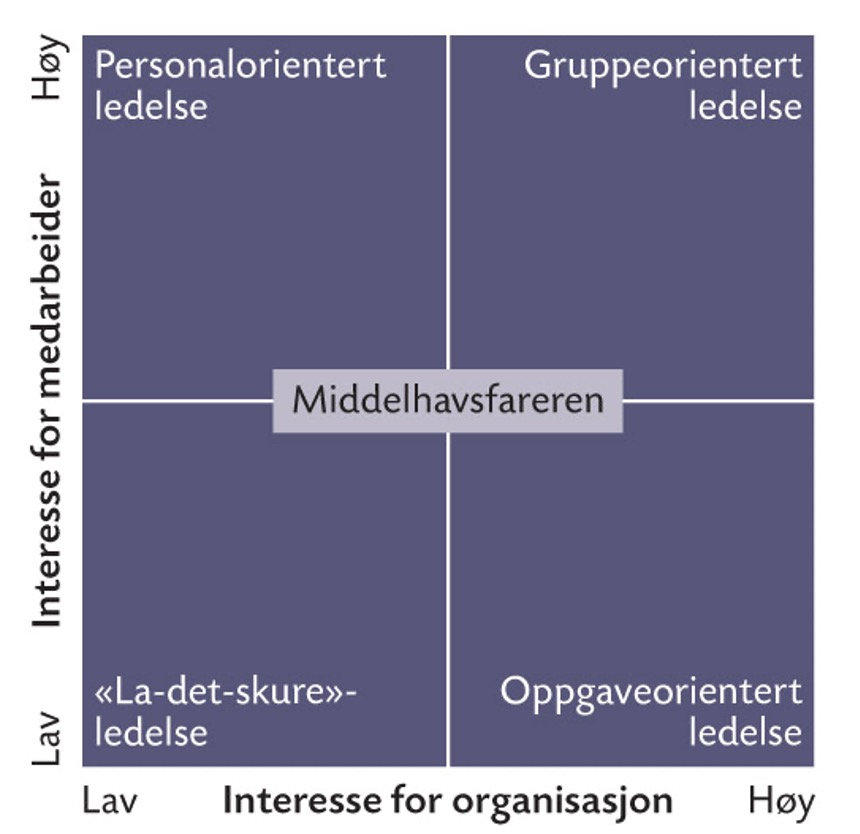
\includegraphics[width=8cm]{img/ledergitteret.jpg}
  \caption{Ledergitteret \parencite[63]{ledelse}}
  \label{fig:ledergitter}
\end{figure}

En leder som følger ``La-det-skure''-ledelse vil neppe føle noen store problemer eller utfordringer med en quiet quitter. 
Lederen bryr seg nemlig i praksis lite om medarbeiderne og like lite om bedriftens resultater \parencite{ledelse}. 
At en medarbeider bare gjør akkurat det de blir bedt om og ikke noe mer er jo midt i blinken! 
``Hva skal jeg si, du gjør jo akkurat det jeg ber deg om og ikke noe mer! Hva annet kan jeg forvente'' kan man tenke seg lederen vil si under en medarbeidersamtale.

Den rake motsetningen finner vi ikke overraskende i motsatt felt i gitteret, den gruppeorienterte lederen; 
en leder som er veldig motivert til å oppnå gode resultater, og motivere sine medarbeidere. Her kan det oppstå store gnister under en medarbeidersamtale med en quiet quitter. Lederen kan oppfatte medarbeideren som lat og uinteressert, og medarbeideren kan oppfatte lederen som påtrengende og slitsom.

I samme båt, men på hver sin ende, finner vi den personalorienterte og den oppgaveorienterte lederen. Disse lederne vil oppleve liknende utfordringer som den gruppeorienterte lederen, men må håndtere de ulikt. Den personalorienterte lederen vil kunne oppleve medarbeideren uinteressert i unødvendig samarbeid, og 

\subsection{Hvordan skal en leder forholde seg til Quiet quitting?}


\subsection{Hvordan leder man en Quiet quitter?}


Og kanskje var det nettopp det å gi slipp på arbeidets plikter som var Sinatras amerikanske drøm, ``\emph{Start spreading the news, I'm leaving today}''. Alt han ville var å være fri å gjøre det han ville uten å engste seg over alle andre bekymringer, ``\emph{I want to be a part of it: New York, New York}''.

\newpage
\section{Truer Quiet quitting organisasjonskulturen?}

\newpage
\printbibliography[heading=bibintoc] % LAGER BIBLIOGRAFI

\end{document}
